

  In the diagram, the line represents a direct variation. Which of the following is the value of the constant $a$?

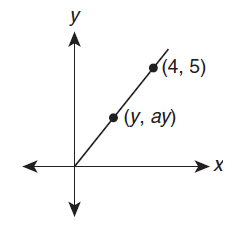
\includegraphics[]{support/Capture11.png}



\ifsat
	\begin{enumerate}[label=\Alph*)]
		\item   1
		\item  4/5
		\item  5/4%
		\item  5
	\end{enumerate}
\else
\fi

\ifacteven
	\begin{enumerate}[label=\textbf{\Alph*.},itemsep=\fill,align=left]
		\setcounter{enumii}{5}
		\item   1
		\item  1/5
		\item  4/5
		\addtocounter{enumii}{1}
		\item  5/4%
		\item  5
	\end{enumerate}
\else
\fi

\ifactodd
	\begin{enumerate}[label=\textbf{\Alph*.},itemsep=\fill,align=left]
		\item   1
		\item  1/5
		\item  4/5
		\item  5/4%
		\item  5
	\end{enumerate}
\else
\fi

\ifgridin
  5/4%
		
\else
\fi

